\section{Microservice Architecture}

The microservice architectural style is an approach to developing a single application as a suite of small services, each running in its own process and communicating with lightweight mechanisms, often an HTTP resource API. These services are built around business capabilities and independently deployable by fully automated deployment machinery. There is a bare minimum of centralized management of these services, which may be written in different programming languages and use different data storage technologies \cite{LewisMicroservices}.

Among the characteristics of \acrfull{microservice}, few characteristics heavily affect while moving from \acrshort{soa} to \acrshort{microservice}.
%%%%%%%%%%%%%%%%%%%%%%%%%%%%%%%%%%%%%%%%%%%%%%%%%%%%%%%%%%%%%%%%%%%%%%%%%%%%%%%%
\subsection{Smart Endpoints And Dumb Pipes}
\label{subse:smart_endpoints}
When building communication endpoints, many architecture approach with putting significant smart into the communication mechanism. One good example is \acrshort{esb} what we discussed in section \ref{se:architectural_decisions}. But microservice follows alternative approach: \emph{Smart endpoints and dumb pipes} \cite{LewisMicroservicesPipes}.
Applications built from microservices aim to be as decoupled and as cohesive as possible. They own their own domain logic and act more as filters in the classical Unix sense. After receiving a request, applying logic as appropriate and producing a response. And it uses simple RESTish protocols rather than complex protocols.

%%%%%%%%%%%%%%%%%%%%%%%%%%%%%%%%%%%%%%%%%%%%%%%%%%%%%%%%%%%%%%%%%%%%%%%%%%%%%%%%
\subsection{Pattern: Database per Service}
\label{subse:database_per_service}
- Pattern: Database per service 

\acrshort{microservice} prefer letting each service manages its own database, either different instances of the same database technology, or entirely different database systems - an approach called \emph{Polyglot Persistence} \cite{LewisMicroservicesManagement}.

Keep each microservice’s persistent data private to that service and accessible only via its API. 
There are a few different ways to keep a service’s persistent data private. You do not need to provision a database server for each service. For example, if you are using a relational database then the options are \cite{RichardsonMicroservicesService}:
\begin{itemize}
    \item \emph{Private-tables-per-service} – each service owns a set of tables that must only be accessed by that service
    \item \emph{Schema-per-service} – each service has a database schema that’s private to that service
    \item \emph{Database-server-per-service} – each service has its own database server.
\end{itemize}
Private-tables-per-service and schema-per-service have the lowest overhead. Using a schema per service is appealing since it makes ownership clearer. Some high throughput services might need their own database server.

%%%%%%%%%%%%%%%%%%%%%%%%%%%%%%%%%%%%%%%%%%%%%%%%%%%%%%%%%%%%%%%%%%%%%%%%%%%%%%%%
\subsection{Pattern: Sagas}
\label{subse:sagas}
In order to ensure loose coupling, each service has its own database. Maintaining data consistency between services is a challenge because 2 phase-commit/distributed transactions is not an option for many applications. An application must instead use the Saga pattern. A service publishes an event when its data changes. Other services consume that event and update their data \cite{RichardsonMicroservicesSagas}.

%%%%%%%%%%%%%%%%%%%%%%%%%%%%%%%%%%%%%%%%%%%%%%%%%%%%%%%%%%%%%%%%%%%%%%%%%%%%%%%%
\subsection{The Scale Cube}
\label{subse:scale_cube}
The microservice architecture is an application of Y-axis scaling but let’s also look at X-axis and Z-axis scaling.

\subsubsection{X-axis Saling}
X-axis scaling consists of running multiple copies of an application behind a load balancer. If there are N copies then each copy handles 1/N of the load. This is a simple, commonly used approach of scaling an application.
One drawback of this approach is that because each copy potentially accesses all of the data, caches require more memory to be effective. Another problem with this approach is that it does not tackle the problems of increasing development and application complexity.

\subsubsection{Y-axis Scaling}
Unlike X-axis and Z-axis, which consist of running multiple, identical copies of the application, Y-axis axis scaling splits the application into multiple, different services. Each service is responsible for one or more closely related functions. There are a couple of different ways of decomposing the application into services.
verb-based decomposition ex: checkout
decompose the application by noun ex: customer management. 
An application might use a combination of verb-based and noun-based decomposition.

\subsubsection{Z-axis Scaling}
When using Z-axis scaling each server runs an identical copy of the code (similar to X-axis scaling). The big difference is that each server is responsible for only a subset of the data. 

Some component of the system is responsible for routing each request to the appropriate server. Ex;
One commonly used routing criteria is an attribute of the request such as the primary key of the entity being accessed. 
Another common routing criteria is the customer type. For example, an application might provide paying customers with a higher SLA than free customers by routing their requests to a different set of servers with more capacity.

Z-axis splits are commonly used to scale databases. Data is partitioned (a.k.a. sharded) across a set of servers based on an attribute of each record. (Ex: the primary key of the RESTAURANT table is used to partition the rows between two different database servers)

Note that X-axis cloning might be applied to each partition by deploying one or more servers as replicas/slaves. Z-axis scaling can also be applied to applications.
(Example of apply Z-axis scaling: the search service consists of a number of partitions. A router sends each content item to the appropriate partition, where it is indexed and stored. A query aggregator sends each query to all of the partitions, and combines the results from each of them.)

%%%%%%%%%%%%%%%%%%%%%%%%%%%%%%%%%%%%%%%%%%%%%%%%%%%%%%%%%%%%%%%%%%%%%%%%%%%%%%%%
\subsection{Brief introduction to the \acrfull{k8s}}
\label{sebse:k8s_intro}

\begin{figure}[htp]
    \centering
    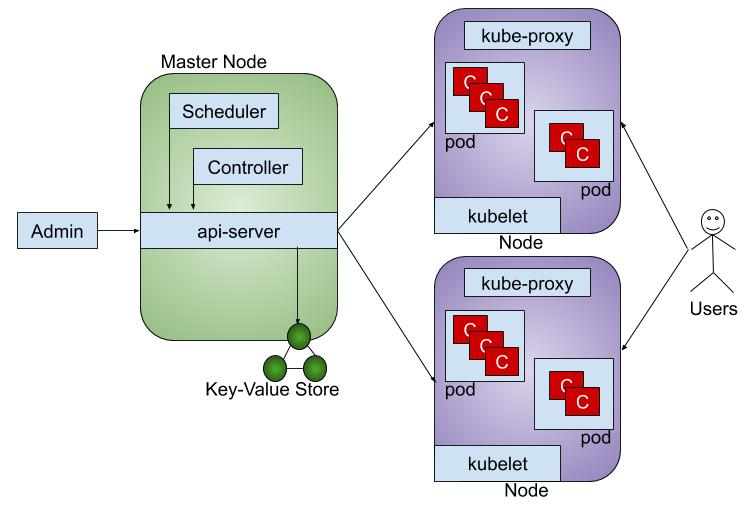
\includegraphics[width=1\textwidth]{method/microservice/k8s_architecture_v3.jpg}
    \caption{\acrfull{k8s} architecture.}
    \label{fi:k8s_architecture}
\end{figure}

- Explain how k8s support microservice architecture

<explain how each one is used while designing the WDIAS architecture>

\begin{figure}[htp]
    \centering
    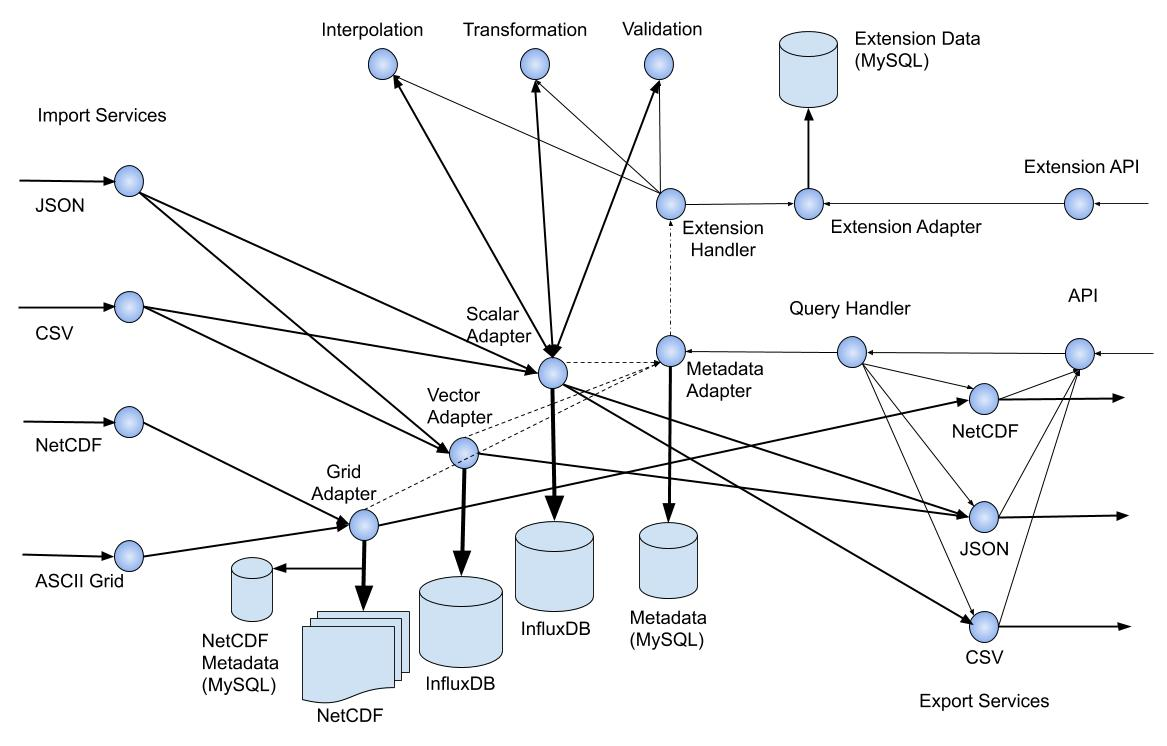
\includegraphics[width=1\textwidth]{method/microservice/microservice_architecture-handle_on_demand-v3.jpg}
    \caption{\acrshort{wdias} architecture for server requests on demand}
    \label{fi:wdias_micro_on_demand}
\end{figure}

\begin{figure}[htp]
    \centering
    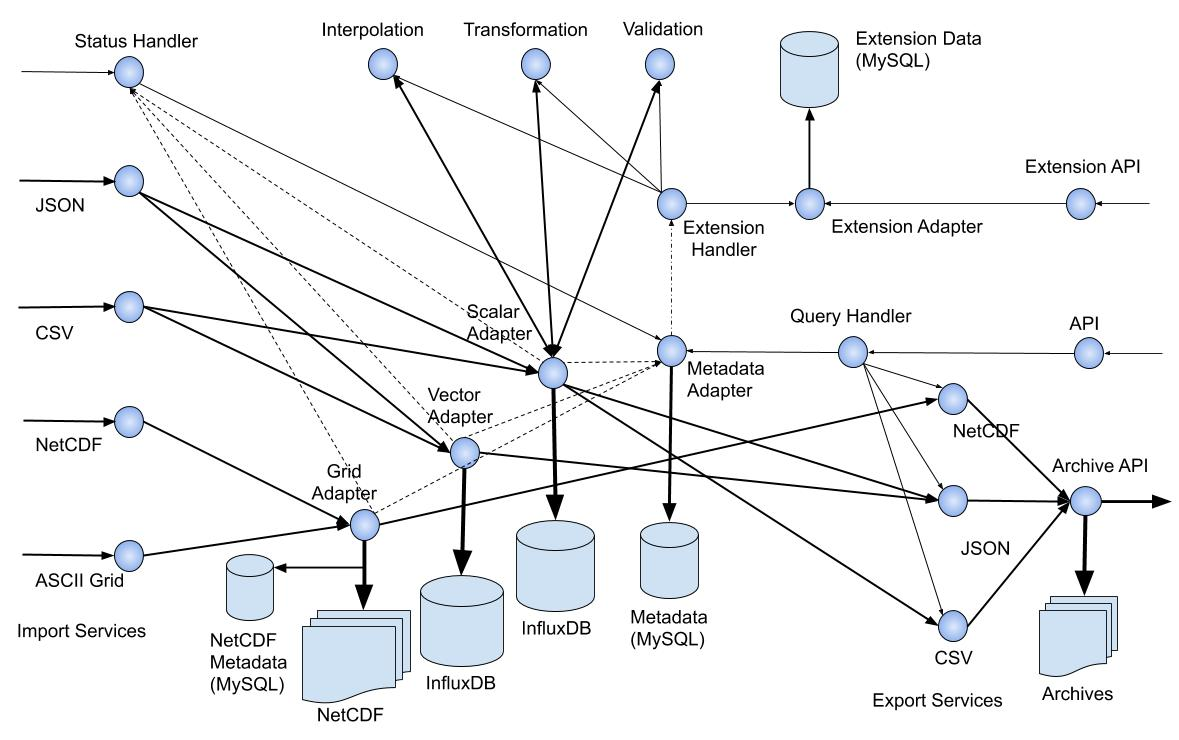
\includegraphics[width=1\textwidth]{method/microservice/microservice_architecture-handle_on_async-v3.jpg}
    \caption{\acrshort{wdias} architecture for handle request asynchronously}
    \label{fi:wdias_micro_async}
\end{figure}

\begin{figure}[htp]
    \centering
    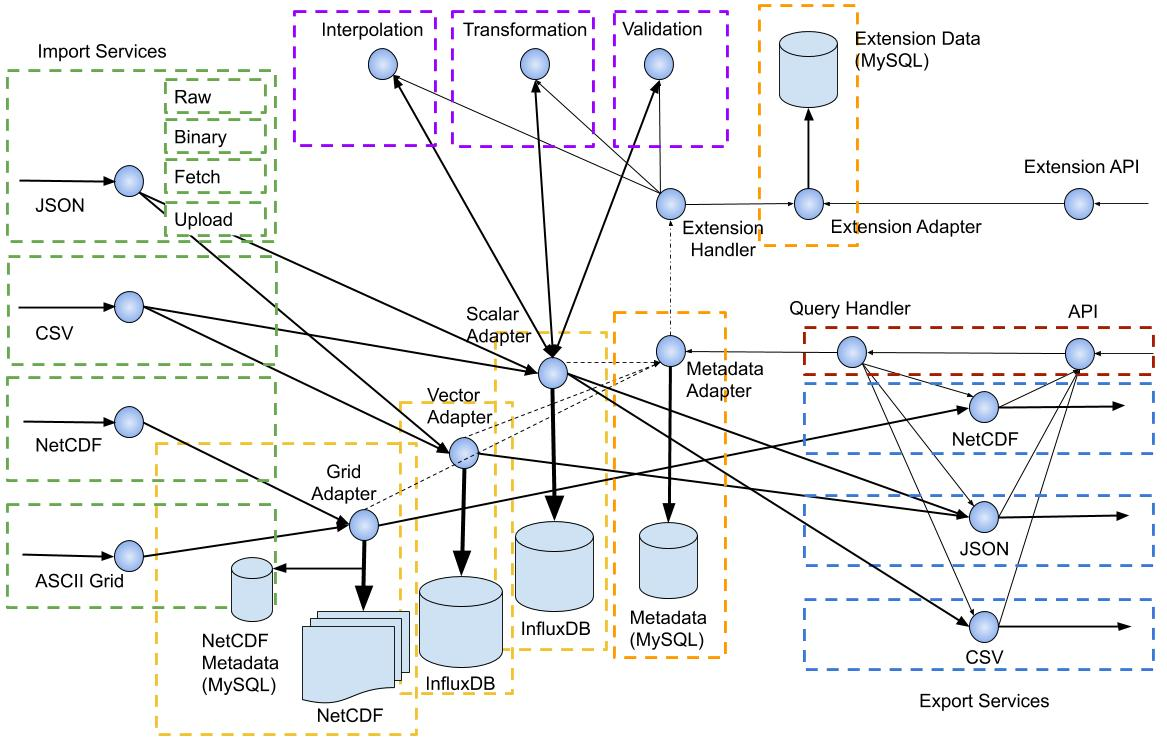
\includegraphics[width=1\textwidth]{method/microservice/separation_microservices-v3.jpg}
    \caption{Separation \acrshort{wdias} microservices}
    \label{fi:wdias_micro_separation}
\end{figure}

<add the API description and how it related to modules>
- Import
- Export
- Timeseries
- Extensions
